\chapter{РЕАЛИЗАЦИЯ}

\section{Программное обеспечение КУСД}

Работа КУСД, как было сказано ранее (стр. \pageref{reasonofwork}), полностью зависит от поддержки стека сетевых протоколов TCP/IP. Следовательно, основная часть данной работы направлена на создание программного обеспечения, реализующего поддержку стека сетевых протоколов.

В качестве инструмента реализации программного обеспечения использовался домашний компьютер с ОС Linux Ubuntu 16.04, на котором было установлен следующее ПО:
 \begin{itemize}
	\item набор GNU AVR Toolchain версии 4.9.2, в который входит\cite{avrtoolchain}:
	\begin{itemize}
		\item[•] компилятор avr-gcc, для комплиляции исходного кода на языке С/С++ в машинный язык микроконтроллеров семейства AVR;
		\item[•] набор ассемблера и компоновщика avr-binutils;
		\item[•] avr-libc --- подмножество стандартной библиотеки С с некоторыми специфичными для AVR функциями;
		\item[•] avr-gdb --- отладчик;
		\item[•] avrdude --- программа для загрузки/выгрузки/управления памятью программ и данных на МК AVR;
	\end{itemize}
	\item интегрированная среда разработки Elcipse версии 3.8.1 с плагином для разработки программ на МК AVR;
\end{itemize}

\section{Работа с Ethernet-контроллером}

Первоначально требовалось обеспечить передачу данных между Ethernet-контроллером и микроконтроллером ATmega328/P по шине SPI. Опираясь на таблицу \ref{spitabl}, а также на расположение выводов контроллера ENC28J60 (рисунок \ref{fig:ethcontroller}), микроконтроллер был подключен к Ethernet-контроллеру. Соответствие выходам микроконтроллера ATmega328/P и входам Ethernet-контроллера описано в таблице \ref{connection}. Стоит отметить что хоть Ethernet-контроллер в основном оперирует напряжением 3,3 В, на вход питания можно подавать 5 В и выше, поскольку на плате присутствует стабилизатор напряжения AMS1117\cite{voltageregulator}. После подключение убеждаемся в том, что на плату Ethernet-контроллера поступает питание по свечению светодиода D1. 

\begin{table}[h!]
\caption{Соответствие выходам ATmega328/P и входам Ethernet-контроллера в данной работе}
\label{connection}
	\begin{tabular}{|p{40mm}|p{40mm}|p{40mm}|}
\hline
	Наименование соединения & Выход на ATmega328/P & Вход на Ethernet-контроллере \\
\hline
		MOSI & PB3 & MOSI (4)\\
\hline
		MISO & PB4 & MISO(10)\\
\hline
		SCLK & PB5 & SCK(9)\\
\hline
		SS & PB2 & CS (5)\\
\hline
\end{tabular}
\end{table}

Для взаимодействия с Ethernet-контроллером была написана библиотека на языке Си. Здесь и далее форматы заголовков различных протоколов будут описываться структурами данных на языке Си. Заранее определим используемые типы и определения:
\begin{itemize}
	\item типы:
	\begin{itemize}
		\item[•] \textit{uint8\_t} --- беззнаковое целое число, 8 бит;
		\item[•] \textit{uint16\_t} --- беззнаковое целое число, 16 бит;
		\item[•] \textit{uint32\_t} --- беззнаковое целое число, 32 бита;
	\end{itemize}
	\item определения:
	\begin{itemize}
		\item[•] \textit{htons(a)} --- макрос, обеспечивающий перевод порядка байтов, принятого у данного хоста, к сетевому (2 байта);
		\item[•] \textit{htonl(a)} --- макрос, обеспечивающий перевод порядка байтов, принятого у данного хоста, к сетевому (4 байта);
		\item[•] \textit{ntohs(a)} --- макрос, обеспечивающий перевод от сетевого порядка байтов до порядка, принятого у данного хоста (2 байта);
		\item[•] \textit{ntohl(a)} --- макрос, обеспечивающий перевод от сетевого порядка байтов до порядка, принятого у данного хоста (4 байта);
	\end{itemize}
\end{itemize}

Основной интерфейс данной библиотеки представлен в листинге \ref{lst:enc28j60header}. 

{\small{\lstinputlisting[language=C, caption=Интерфейс для взаимодействия с ENC28J60 по шине SPI\label{lst:enc28j60header}, inputencoding=cp1251, linerange={12-33}]{./src/enc28j60.h}}}

Алгоритм работы с Ethernet-контроллером следующий:
\begin{enumerate}
	\item настраиваем работу по шине SPI: 
		\begin{itemize}
			\item конфигурируем выходы микроконтроллера CS, MOSI, SCK на запись, а MISO на чтение;
			\item устанавливаем режим работы SPI интерфейса ATmega328/P как ``Мастер'';
			\item выставляем скорость работы шины SPI на максимальную;
			\item используем SPI режим 0 (CPOL=0, CPHA=0);
		\end{itemize}
	\item инициализируем ENC28J60:
		\begin{itemize}
			\item делаем ``мягкий сброс'' микросхемы;
			\item устанавливаем размер FIFO для приема данных (ERXST, ERXND), инициализируем указатель для чтения данных из FIFO (ERXRDPT);
			\item конфигурируем MAC: включаем аппаратное управление потоком, автоматическое выравнивание до 60 байт, автоматическое добавление контрольной суммы, устанавливаем MAC-адрес в регистрах MAADR;
			\item настраиваем PHY: устанавливаем дуплексный режим, настраиваем индикаторные светодиоды, отключаем loopback;
			\item разрешаем прием пакетов;
		\end{itemize}
	\item принимаем и отправляем пакеты;
\end{enumerate}

После того, как мы получили возможность обмениваться сырыми данными с другими Ethernet-устройствами, осталось написать протоколы канального, сетевого и транспортного уровня.

\section{Реализация протоколов стека TCP/IP}

\subsection{Ethernet}

Заголовки протокола Ethernet представлены в листинге \ref{lst:ethernethead}. 

{\small{\lstinputlisting[language=C, caption=Определение полей и заголовков для манипулирования Ethernet-кадрами\label{lst:ethernethead}, inputencoding=cp1251, linerange={13-13, 41-49}]{./src/lan.h}}}

Далее требовалось реализовать поддержку протокола сетевого уровня IP, что бы успешно взаимодействовать с другими хостами в сети, построенной на базе стека протоколов TCP/IP.

\subsection{IP}

\textbf{IP} (\textit{Internet Protocol}) ~--- протокол, реализующий основу транспортных средств стека протоколов TCP/IP. Является базовым элементом технологии Internet, а таблица маршрутов ~--- центральная часть этого протокола. Каждый хост в IP-сети имеет свой уникальный идентификатор ~--- так называемый, \textit{IP-адрес}, который может быть получен различными способами. Он может быть присвоен статически или динамически. Длина IP-адреса --- 4 байта. Стоит отметить, что этот адрес идентифицирует точку доступа модуля IP к сетевому интерфейсу, а не всю машину целиком.

Стоит подробнее рассмотреть таблицу маршрутизации, которая хранится в КУСД. Данная таблица описывает соответствие между адресами назначения и интерфейсами, через которые следует отправить пакет данных до следующего маршрутизатора \cite{ip}. Она обычно содержит:
\begin{itemize}
	\item[•] \textit{Destination} --- адрес сети или узла назначения, либо указание, что маршрут является маршрутом по умолчанию;
	\item[•] \textit{Netmask} --- маска сети назначения;
	\item[•] \textit{Gateway}, или \textit{Next Hop} --- следующий маршрутизатор;
	\item[•] \textit{Interface} --- интерфейс (численный или символьный идентификатор устройства);
	\item[•] \textit{Metric} --- число, соответствующее предпочтительности маршрута (чем число меньше, тем более предпочтителен маршрут);
\end{itemize}

Поскольку в данной работе имеется только макет КУСД и нет цели использовать все возможности таблицы маршрутизации, используется информация о маске подсети в которой находится КУСД, его IP-адрес и стандартный маршрутизатор. Заголовки протокола IP и таблица маршрутизации представлены в листинге \ref{lst:iphead}.

{\small{\lstinputlisting[language=C, caption=Определение полей и заголовков для манипулирования IP-датаграммами\, таблица маршрутизации\label{lst:iphead}, inputencoding=cp1251, linerange={14-18, 83-100}]{./src/lan.h}}}

\subsection{ARP}

После того как определен и реализован некоторый базис, позволяющий передавать пакеты в локальной сети, необходимо связать канальный и сетевые уровни протоколом \textbf{ARP} (\textit{Address Resolution Protocol})\cite{arp}. Это необходимо поскольку не существует другого явного алгоритма преобразования IP-адрес в MAC-адреса\cite{arpcitforum}.

Рассмотрим процедуру преобразования адресов при отправлении сообщения. Пусть один хост отправляет сообщение другому. Прикладной программе IP-адрес места назначения обычно известен. Для определения MAC-адреса просматривается ARP-таблица. Если для требуемого IP-адреса в ней присутствует MAC-адрес, то формируется и посылается пакет по соответствующему адресу. Если же с помощью APR-таблицы не удается преобразовать адрес, то выполняется следующее:
\begin{itemize}
	\item всем хостам в сети посылается пакет с ARP-запросом (с широковещательным MAC-адресом);
	\item исходящий IP-пакет ставится в очередь;
\end{itemize}

Каждый хост, принявший ARP-запрос, в своем ARP-модуле сравнивает собственный IP-адрес с IP-адресом в запросе. Если IP-адрес совпал, то прямо по MAC-адресу отправителя запроса посылается ответ, содержащий как IP-адрес ответившей машины, так и её MAC-адрес. Далее ответ принимается и заносится в ARP-таблицу, после чего отправляются все IP-пакеты которые были занесены в очередь на отправку к данному хосту. В противном случае (такой машины в сети нет) все IP-адреса по данному адресу отбрасываются. Пример ARP-таблицы отображен в таблице \ref{arptable}.

\begin{table}[h!]
\caption{Пример упрощенной ARP-таблицы}
\label{arptable}
	\begin{tabular}{|c|c|}
	\hline
	IP-адрес & MAC-адрес\\
	\hline
	192.168.0.1 & 30:b5:c2:cd:73:90 \\
	\hline
	192.168.0.102 & f4:f5:a5:73:da:b6 \\
	\hline
	192.168.0.103 & f8:32:e4:34:e7:61 \\
	\hline
	192.168.0.101 & 00:24:21:21:26:72 \\
	\hline
	\end{tabular}
\end{table}

Заголовки протокола ARP представлены в листинге \ref{lst:arphead}.

{\small{\lstinputlisting[language=C, caption=Определение полей и заголовков для протокола ARP\label{lst:arphead}, inputencoding=cp1251, linerange={20-20, 56-78}]{./src/lan.h}}}

\subsection{ICMP}

Для тестирования работоспособности сетевого интерфейса (и вообще КУСД) не будет лишним реализовать поддержку протокола \textbf{ICMP}, а именно ICMP Echo запросы и ответы. Сам протокол ICMP служит для диагностики состояния сети. Echo-запросы имеют следующие поля:
\begin{enumerate}
	\item тип пакета: запрос (8) или ответ (0);
	\item код пакета --- 0 для Echo-запроса и ответа;
	\item контрольная сумма заголовка рассчитывается также, как и для заголовка IP-пакета;
	\item остальные поля устанавливаются на усмотрение хоста. Ответ должен содержать те же значения;
\end{enumerate}

Заголовки протокола ICMP (для Echo-запросов) представлены в листинге \ref{lst:icmpecho}.

{\small{\lstinputlisting[language=C, caption=Определение полей и заголовков для ICMP Echo запросов\label{lst:icmpecho}, inputencoding=cp1251, linerange={106-119}]{./src/lan.h}}}

Убедимся, что контроллер отвечает на Echo-запросы, отправив по его IP-адресу Echo-запрос. При этом, контроллер будет находится в домашней локальной сети по IP-адресу 192.168.0.140 и маской подсети 255.255.255.0. Отправим несколько Echo-запросов используя утилиту \textbf{ping} на одном из хостов в локальной сети (рисунок \ref{fig:echo-req}). При этом, будут считываться сообщения приходящие от самого контроллера по протоколу USART на домашний компьютер (рисунок \ref{fig:echo-reply-log}).

\begin{figure}[h!]
	\centering
		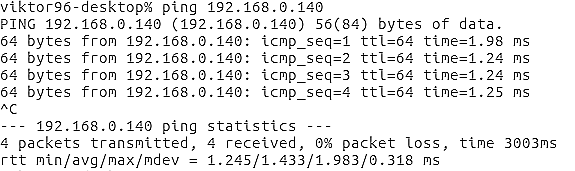
\includegraphics[scale=0.8]{img/icmp-req.png}
	\caption{Отправка Echo-запросов к КУСД\label{fig:echo-req}}
\end{figure}

\begin{figure}[h!]
	\centering
		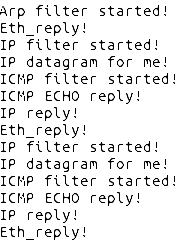
\includegraphics[scale=0.7]{img/echo-reply-log.png}
	\caption{Подтверждения о доставке Echo-запросов и ответа на них\label{fig:echo-reply-log}}
\end{figure}

Данные отладочные сообщают о том, что принятый пакет прошел стадии обработки Ethernet фильтра, где контроллер распознал свой MAC-адрес, следом IP фильтра, где контроллер распознал свой IP-адрес, далее ICMP фильтра, в котором был распознан код и типа сообщения (код Echo-запроса, тип --- запрос). Следом был отправлен Echo-ответ, который последовательно компоновался от уровня ICMP до Ethernet и был послан в сеть.

Как видно из рисунка \ref{fig:echo-req} по тому, что на все запросы были посланы ответы, стек протоколов от Ethernet до ICMP на данном контроллере работоспособен.

\subsection{UDP}

\textbf{UDP} (\textit{User Datagram Protocol}) ~--- простейший протокол транспортного уровня. Используется для отсылки данных некритичных к потере информации приложений. Также UDP используется для рассылки групповых IP датаграмм. Формат UDP заголовка представлен в листинге \ref{lst:udphead}.

{\small{\lstinputlisting[language=C, caption=Определение UDP заголовка\label{lst:udphead}, inputencoding=cp1251, linerange={125-131}]{./src/lan.h}}}

\section{Настройка и взаимодействие КУСД через USART}

В процессе первого монтажа и наладки работы КУСД требуется осуществить настройку его сетевых параметров. Всё это необходимо делать в условиях минимального набора дополнительных инструментов, которые должны быть у монтажника в момент установки и наладки. Было принято решение использовать интерфейс USART для настройки сетевых параметров, а также тестирования работы КУСД. Использование такого распространенного интерфейса позволяет получить доступ к настройкам КУСД, не используя узко-специализированное программное обеспечение. Для повышения безопасности можно снабдить КУСД закрытым паролем, который будет известен только той организации, которой предоставляется информация о состоянии сети. Верификация пароля будет происходить на начальном этапе установления сеанса связи по USART.

Особенностью данного интерфейса взаимодействия является то, он --- текстовый. Текстовый способ взаимодействия, против бинарного, был выбран по следующим причинам:
\begin{enumerate}
	\item это человеко-читаемый интерфейс, а это значит, что он будет понятен;
	\item не требует специальных средств расшифровки бинарных данных;
	\item позволяет использовать любой текстовый USART терминал, что расширяет круг устройств которые могут считывать и посылать на КУСД данные;
\end{enumerate}

Однако такой выбор имеет и недостатки:
\begin{enumerate}
	\item память программ КУСД должна быть достаточно большой (от 8 Кбайт и более) для поддержки текстового интерфейса;
	\item такому интерфейсу свойственны все недостатки текстовых компьютерных интерфейсов: переполнение буфера, опечатки, медлительность работы;
\end{enumerate}

Была написана библиотека на языке Си, для микроконтроллера ATmega328/P, реализующая прием и отправку данных по USART. Её интерфейс отображен в листинге \ref{lst:usartif}.

{\small{\lstinputlisting[language=C, caption=Интерфейс взаимодействия с USART\label{lst:usartif}, inputencoding=cp1251, linerange={17-33}]{./src/usart.h}}}

Далее была написана программа (см. листинг \ref{lst:main}), которая выполняет активный прием и передачу пакетов, а также способная, в режиме реального времени, изменять сетевые конфигурации КУСД. Логику работы программы лучше всего описывает модель конечного автомата. Всего имеется 4 состояния:
\begin{itemize}
	\item прослушка порта;
	\item отображение конфигурации;
	\item настройка конфигурации;
	\item командный режим;
\end{itemize}

Находясь в состоянии "прослушка порта", КУСД принимает все пакеты, которые приходят извне, а также отправляет данные о энергопотреблении удаленному серверу сбора данных. При этом если это ICMP или ARP запросы, то на них немедленно высылаются соответствующие ответы. В состоянии "отображение конфигурации" КУСД отправляет данные о своих сетевых настройках. В режиме настройка конфигурации возможно изменение сетевых параметров контроллера. В командном режиме осуществляется как прием пакетов, так и выполнение некоторого перечня команд, например отправки пакета на определенный адрес (для тестирования). Переход из одного состояния в другой происходит по, приходящим из интерфейса USART, однобайтовым текстовым командам (например символ 'h' - команда для отображения подсказки). Для взаимодействия с контроллером была использована утилита \textbf{picocom v1.7}, она реализует текстовый интерфейс взаимодействия по протоколу USART и другим. Текстовый интерфейс настройки КУСД отображен ниже:

\begin{verbatim}
picocom v1.7

port is        : /dev/ttyUSB0
flowcontrol    : none
baudrate is    : 9600
parity is      : none
databits are   : 8
escape is      : C-a
local echo is  : yes
noinit is      : no
noreset is     : no
nolock is      : no
send_cmd is    : sz -vv
receive_cmd is : rz -vv
imap is        : lfcrlf,
omap is        : 
emap is        : crcrlf,delbs,

Terminal ready
USART: Setup success!
End of initialization enc28j60

STATE: Polling

To start work:
s - view interface settings
c - configure interface settings
d - enter to command mode
l - enable/disable logger
h - help
%>
\end{verbatim}

Рассмотрим установленные текущие сетевые конфигурации, отправив символ-команду 's' (settings):
\begin{verbatim}
%> s
STATE: View

MAC = 0x0013 0x3301 0x2548 
IP = 192.168.0.140
Subnet mask = 255.255.255.0
Default gateway = 192.168.0.1
Server IP = 192.168.0.104

STATE: Polling
\end{verbatim}

Можно увидеть следующие сетевые параметры: MAC-адрес устройства, IP-адрес устройства, маска подсети, шлюз по умолчанию, адрес сервера сбора данных. Рассмотрим, процесс изменения настроек. Допустим нужно изменить IP-адрес сервера на 192.168.0.107. Отправляем символ-команду 'c':

\begin{verbatim}
%> c
STATE: Configure

MAC = 0x0013 0x3301 0x2548 
IP = 192.168.0.140
Subnet mask = 255.255.255.0
Default gateway = 192.168.0.1
Server IP = 192.168.0.104

tap 'q' to quit

change:
i - IP
m - mask
d - default
s - server IP
\end{verbatim}

На выбор предлагается изменить один из параметров. Выберем \textit{server IP}.

\begin{verbatim}
s
Enter address in x.x.x.xs format (s - stop):
\end{verbatim}

Вводим IP-адрес в требуемом формате:

\begin{verbatim}
192.168.0.107s
Configuration successfully seted

MAC = 0x0013 0x3301 0x2548 
IP = 192.168.0.140
Subnet mask = 255.255.255.0
Default gateway = 192.168.0.1
Server IP = 192.168.0.107

tap 'q' to quit

change:
i - IP
m - mask
d - default
s - server IP
\end{verbatim}

КУСД информирует об успешном изменении параметров сети, печатает новые конфигурации и предлагает выбрать следующий вариант настроек. При отправке команды 'q', КУСД вернется в режим приема и передачи пакетов.

Далее отправим тестовый UDP-пакет с сообщением ``Hello! I'm MCU!'' на ``удаленный сервер'' (функция send\_udp\_test в главной программе). ``Удаленным сервером'' будет один из компьютеров в локальной сети. Для этого перейдем в командный режим:

\begin{verbatim}
To start work:
s - view interface settings
c - configure interface settings
d - enter to command mode
l - enable/disable logger
h - help
%> d
STATE: Command mode

tap 'q' to quit

s - send test udp packet to server
\end{verbatim}

И отправим команду 's', которая заставит КУСД выслать тестовый пакет по адресу 192.168.0.107:

\begin{verbatim}
s
Test packet was sent

tap 'q' to quit

s - send test udp packet to server
\end{verbatim}

Видим, что пакет был отправлен. На другом хосте в этот момент работал сниффер (сетевой анализатор трафика) \textbf{tshark}.

\begin{verbatim}
# ---------- На хосте с IP-адресом 192.168.0.107 --------------------
# Перехват приходящих от КУСД пакетов
viktor96-desktop% tshark -f "src host 192.168.0.140" -w dump.pcap 
viktor96-desktop% tshark -r dump.pcap -T fields -e data | perl -e \ 
pipe>  '$hex = (<>)[1]; while($hex =~/(.{2})/sg) {print chr(hex($1))}'
Hello! I'm MCU!		# <-- Сообщение, посланное КУСД поверх UDP
\end{verbatim}

Сообщение было успешно принято, а его содержимое распознано.

На будущее запланирована поддержка протокола DHCP для динамической настройки сетевых параметров, а также написание программного обеспечения для удаленного изменения сетевых параметров (собственный протокол поверх UDP). Дополнительно к этому будут рассмотрены вопросы считывания данных от счетчиков и ввод КУСД в режим пониженного энергопотребления.
